% Beginning of preamble 
\documentclass[12pt]{article}  

\usepackage{amssymb, amsmath, amsthm, amsfonts}
\usepackage{euscript}
\usepackage{graphicx}
\usepackage[dvipsnames]{xcolor}
\usepackage{url}
\usepackage{hyperref}
\hypersetup{colorlinks=true, urlcolor=RoyalBlue, citecolor=RedViolet}
\usepackage{geometry}
\geometry{left=1in, right=1in, top=1in, bottom=1in}
\usepackage{enumitem}
\usepackage{setspace} 
\setlength\parindent{0pt}
\linespread{1.2}

% Define a few theorem-type environments with numbering
\newtheorem{problem}{Problem} % Automatically numbers each problem
\theoremstyle{definition} 
\newtheorem*{answer}{Answer}

% Make the font Helvetica
\usepackage{helvet}
\renewcommand{\familydefault}{\sfdefault}

% Some notation shortcut commands
\newcommand{\R}{\mathbb{R}} 
\newcommand{\Q}{\mathbb{Q}} 
\newcommand{\N}{\mathbb{N}} 
\newcommand{\Z}{\mathbb{Z}} 
\newcommand{\eps}{\varepsilon} 
\newcommand{\solution}{\textcolor{PineGreen}{Solution:\newline}}

%%%%% End of preamble %%%%%
%--------------------------------------------------------------------------

\begin{document}

\begin{center}
\textbf{CSE 5160 Machine Learning} \hfill \textbf{Giovanni Almaraz, Doug Fry, Zachary Hampton}\\
\textbf{Dr. Haiyan Qiao} \hfill \textbf{03-02-2025}
\end{center}

\bigskip

\section*{Group Assignment 3}

\subsection*{Part A (Textbook Chapter 4.8 Exercises: Q1, Q6, Q8)}

\begin{problem}
\textbf{Problem 1:} Using a little bit of algebra, prove that (4.2) is equivalent to (4.3). In other words, the logistic function representation and the logit representation for the logistic regression model are equivalent.
\end{problem}

\begin{answer}
\solution
Let 
\[
p(X) = \frac{1}{1 + e^{-(\beta_0 + \beta_1 X)}}.
\]
We want to show this is equivalent to
\[
\log\left(\frac{p(X)}{1 - p(X)}\right) = \beta_0 + \beta_1 X.
\]
\textbf{Proof:}

\[
p(X) = \frac{1}{1 + e^{-z}}, \quad \text{where } z = \beta_0 + \beta_1 X.
\]
Then
\[
1 - p(X) 
= 1 - \frac{1}{1 + e^{-z}}
= \frac{1 + e^{-z} - 1}{1 + e^{-z}}
= \frac{e^{-z}}{1 + e^{-z}}.
\]
Hence,
\[
\frac{p(X)}{1 - p(X)} 
= \frac{\frac{1}{1 + e^{-z}}}{\frac{e^{-z}}{1 + e^{-z}}}
= \frac{1}{e^{-z}} 
= e^z.
\]
Taking the natural logarithm on both sides,
\[
\log\left(\frac{p(X)}{1 - p(X)}\right) = \log(e^z) = z = \beta_0 + \beta_1 X.
\]
Thus, \((4.2)\) and \((4.3)\) are indeed equivalent.
\end{answer}

\setcounter{problem}{5}
\begin{problem}
\textbf{Problem 6:} Logistic Regression Probability Estimate
\end{problem}

\begin{answer}
\solution
\textbf{(a)} Given that \(\beta_0 = -6\), \(\beta_1 = 0.05\), and \(\beta_2 = 1\), we estimate the probability of getting an A for a student studying 40 hours with a GPA of 3.5 as follows:
\[
    P(Y=1) 
    = \frac{1}{1 + e^{-(-6 + 0.05 \cdot 40 + 1 \cdot 3.5)}} 
    = \frac{1}{1 + e^{-(-6 + 2 + 3.5)}} 
    = \frac{1}{1 + e^{-0.5}} 
    \approx 0.378 \ (\text{37.8\%}).
\]

\textbf{(b)} To find the number of hours a student with a GPA of 3.5 needs to study to have a 50\% chance of getting an A, we set $P(Y=1) = 0.5$ and solve for $X_1$:
\[
0.5 = \frac{1}{1 + e^{-(-6 + 0.05 \cdot X_1 + 1 \cdot 3.5)}}
\]

Simplifying:
\[
\begin{aligned}
0.5(1 + e^{-(-6 + 0.05 \cdot X_1 + 3.5)}) &= 1 \\
1 + e^{-(-6 + 0.05 \cdot X_1 + 3.5)} &= 2 \\
e^{-(-6 + 0.05 \cdot X_1 + 3.5)} &= 1 \\
-(-6 + 0.05 \cdot X_1 + 3.5) &= 0 \\
6 - 0.05 \cdot X_1 - 3.5 &= 0 \\
2.5 - 0.05 \cdot X_1 &= 0 \\
-0.05 \cdot X_1 &= -2.5 \\
X_1 &= \frac{2.5}{0.05} = 50
\end{aligned}
\]

Therefore, the student would need to study 50 hours to have a 50\% chance of getting an A in the class.
\end{answer}

\setcounter{problem}{7}
\begin{problem}
\textbf{Problem 8:} Comparison of Logistic Regression and K-Nearest Neighbors
\end{problem}

\begin{answer}
\solution
We have two classification methods:

\begin{enumerate}
    \item \textbf{Logistic Regression:}
    \begin{itemize}
        \item Training error: 20\%
        \item Test error: 30\%
    \end{itemize}
    
    \item \textbf{1-Nearest Neighbor (K=1):}
    \begin{itemize}
        \item Average error: 18\%
    \end{itemize}
\end{enumerate}

Even though KNN (K=1) has a lower average error, it is prone to overfitting and does not generalize well. Logistic regression, despite having a higher test error, is more stable and interpretable.

Thus, logistic regression is the better choice for classifying new observations in this case. However, using a better K value (e.g., K=5 or K=10) for KNN might improve its performance.
\end{answer}

\subsection*{Part B (Stock Market Data: Logistic Regression \& LDA)}

\setcounter{problem}{0}
\begin{problem}
\textbf{Problem 1:} (a)--(d) Logistic Regression on the Stock Market Data
\end{problem}

\begin{answer}
\solution
\begin{itemize}
    \item[(a)] Compute the testing error rate using all predictors \(\text{Lag1}, \text{Lag2}, \text{Lag3}, \text{Lag4}, \text{Lag5}\).
    \item[(b)] Identify which predictors can be removed to reduce the testing error (based on p-values or other criteria).
    \item[(c)] Recompute the testing error after removing the less significant predictors.
    \item[(d)] Given \(\text{Lag1} = 2.1\) and \(\text{Lag2} = -0.5\), calculate the predicted probability of the market going up.
\end{itemize}
\end{answer}

\setcounter{problem}{1}
\begin{problem}
\textbf{Problem 2:} (a)--(c) LDA on the Stock Market Data
\end{problem}

\begin{answer}
\solution
\begin{itemize}
    \item[(a)] Calculate \(\Pr(Y = \text{UP})\) and \(\Pr(Y = \text{DOWN})\) based on the training set.
    \item[(b)] Compute the mean vector of \(\mathbf{X}\) (the predictors) for each class (UP vs. DOWN).
    \item[(c)] Discuss whether using a 70\% posterior probability threshold (\(\Pr(Y=\text{UP}|\mathbf{X}=x) \ge 0.70\)) is feasible or advisable for predicting a market increase.
\end{itemize}
\end{answer}

\newpage

\subsection*{Appendix: Screenshots}

\begin{figure}[htbp]
    \centering
    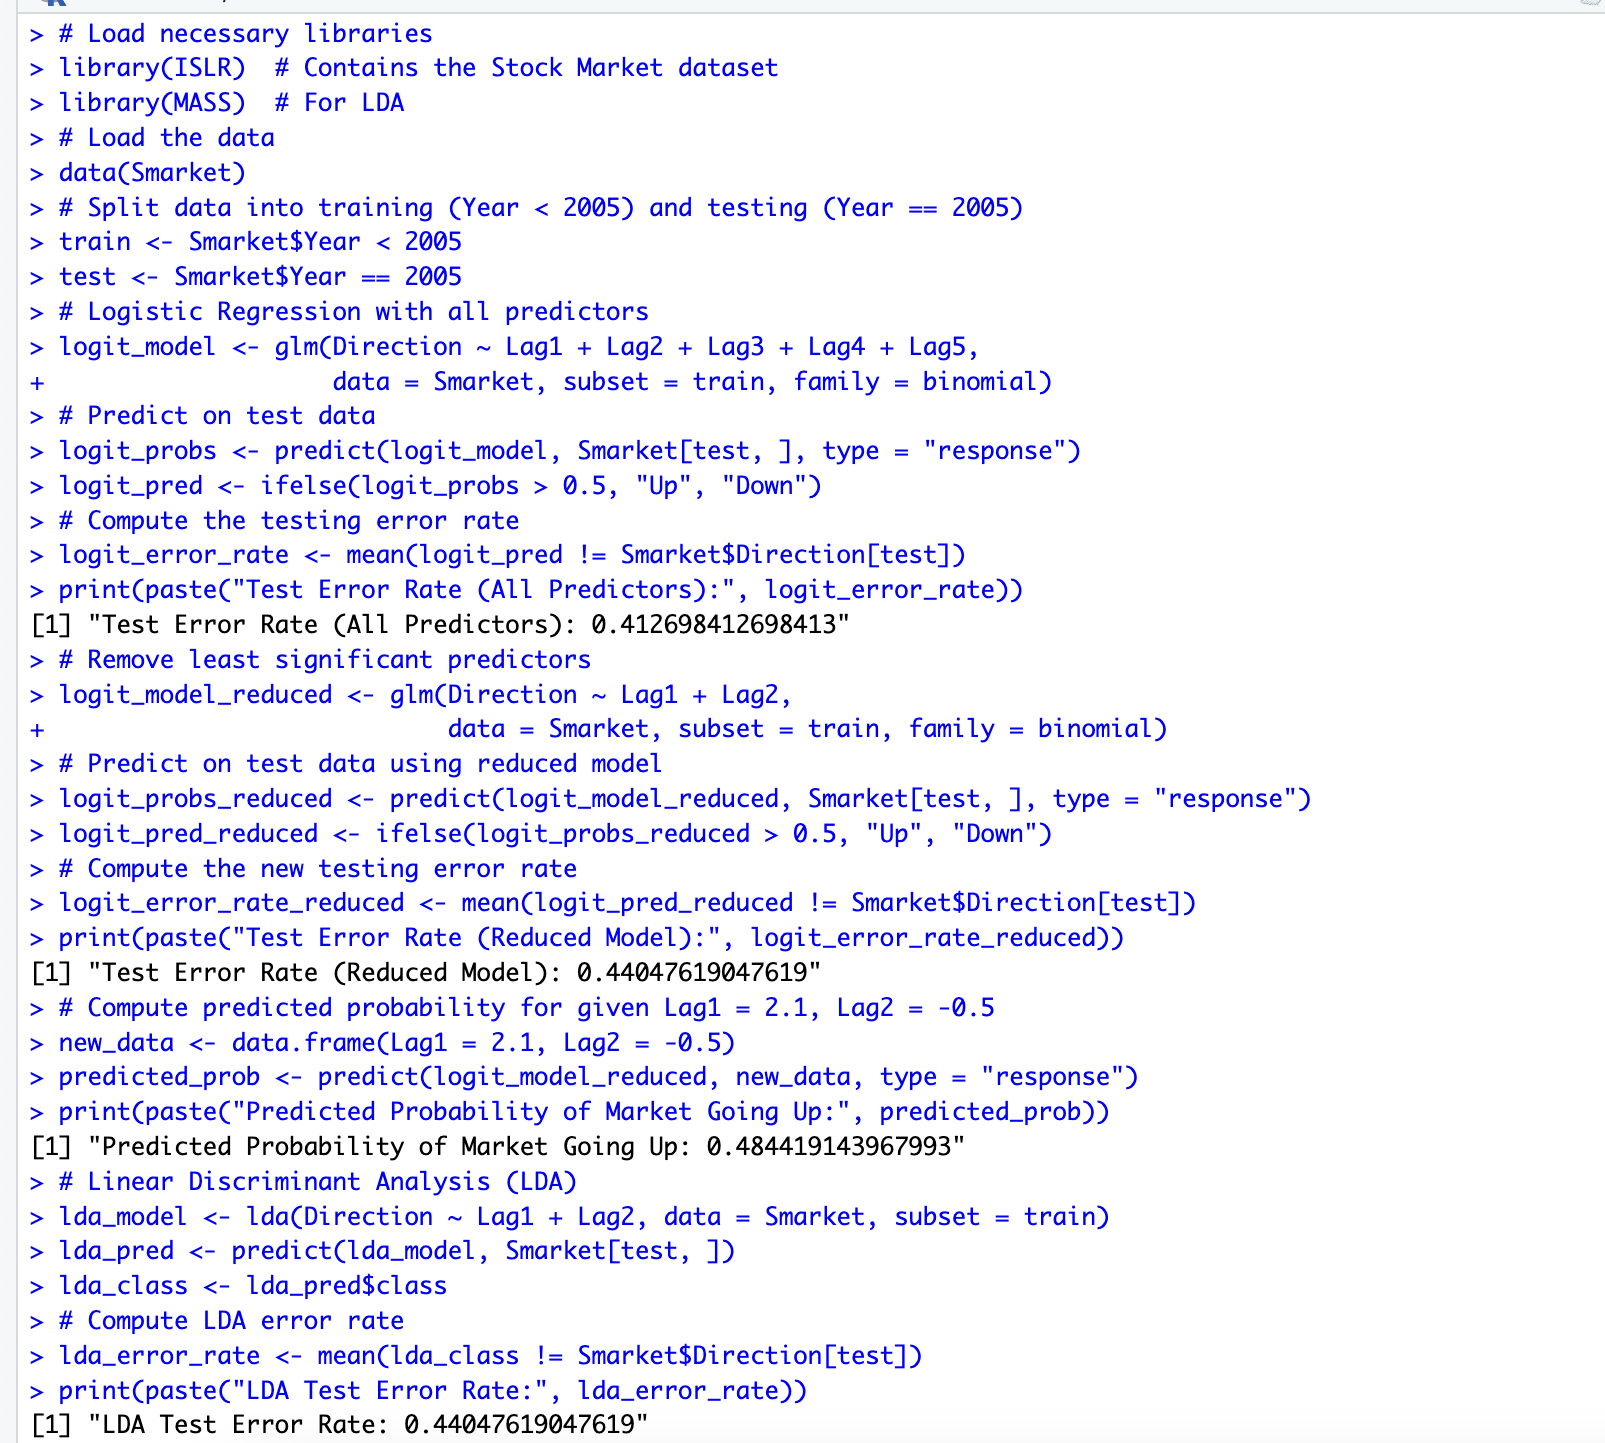
\includegraphics[width=0.85\textwidth]{Screenshot_2025-03-02_at_3.56.05_PM.png}
    \caption{Screenshot 1}
    \label{fig:screenshot1}
\end{figure}

\begin{figure}[htbp]
    \centering
    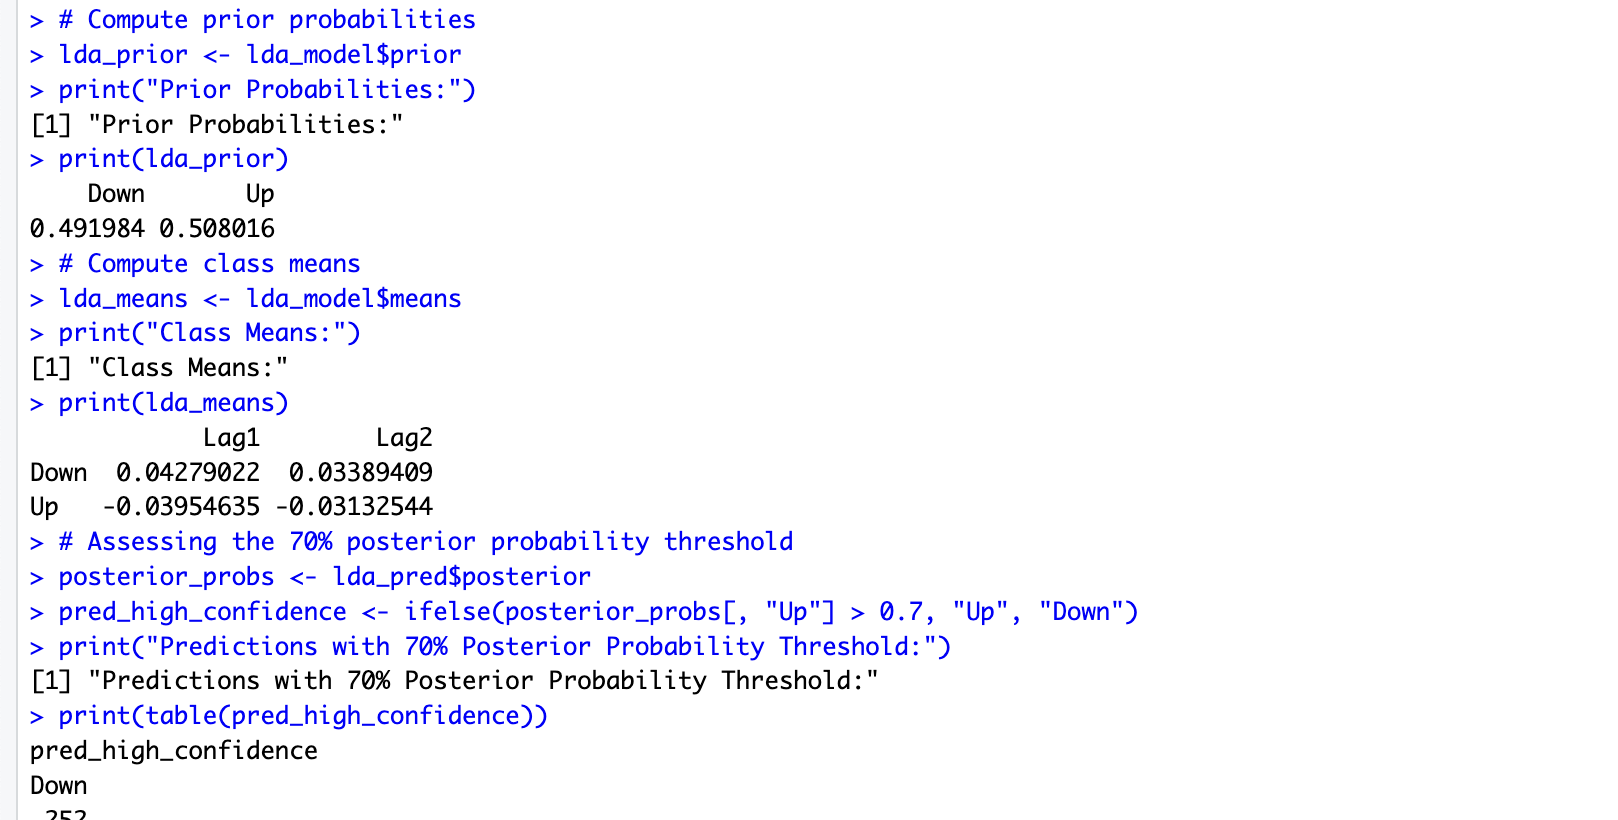
\includegraphics[width=0.85\textwidth]{Screenshot_2025-03-02_at_3.56.32_PM.png}
    \caption{Screenshot 2}
    \label{fig:screenshot2}
\end{figure}

\begin{figure}[htbp]
    \centering
    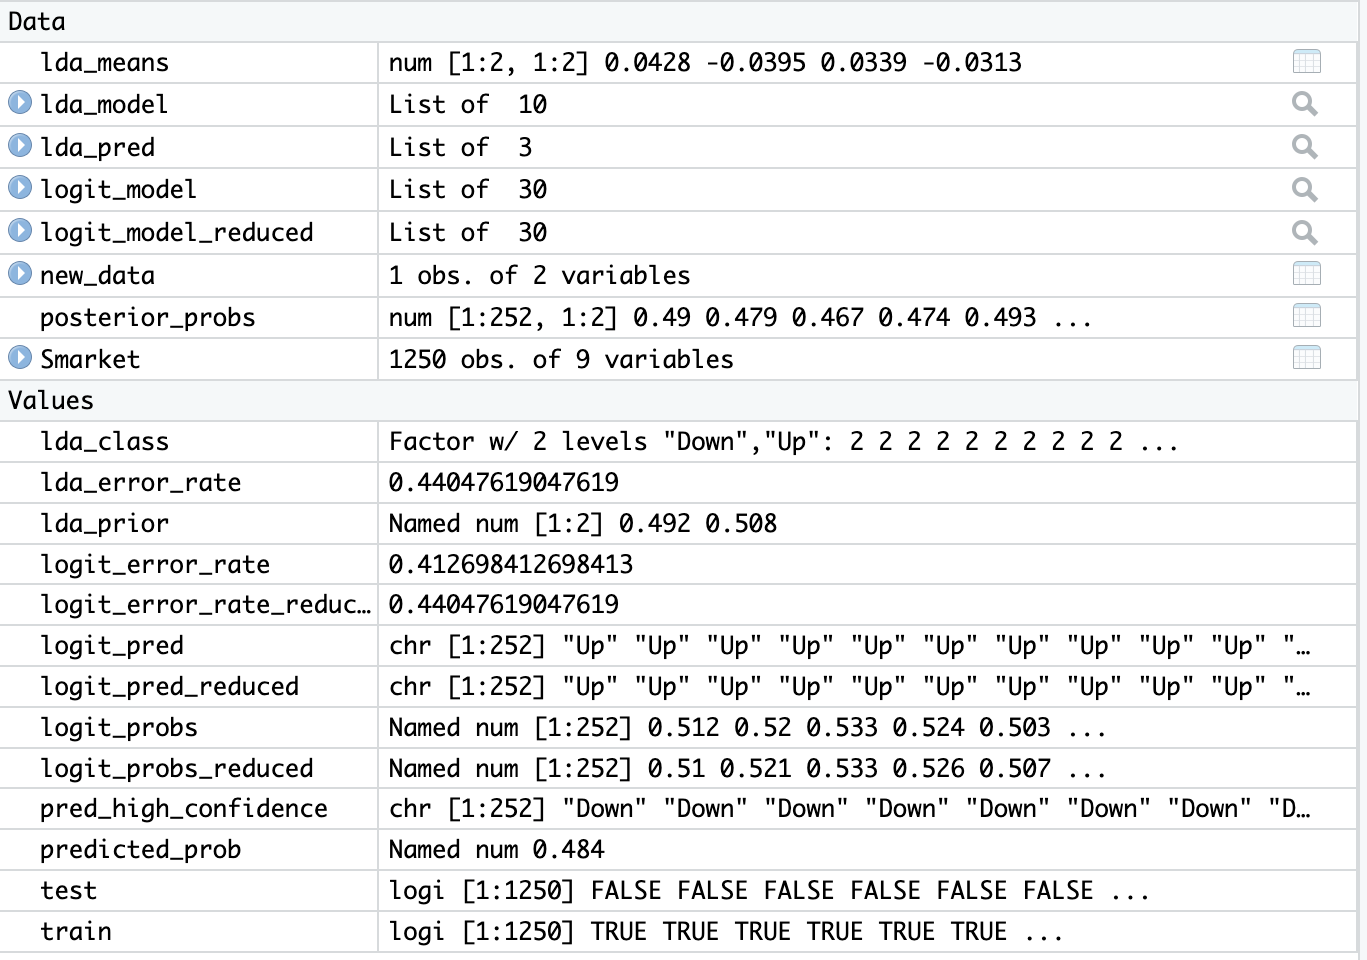
\includegraphics[width=0.85\textwidth]{Screenshot_2025-03-02_at_3.56.51_PM.png}
    \caption{Screenshot 3}
    \label{fig:screenshot3}
\end{figure}

\end{document}